%!TEX root = ../../main.tex


\begin{figure}[!htb]
\centering
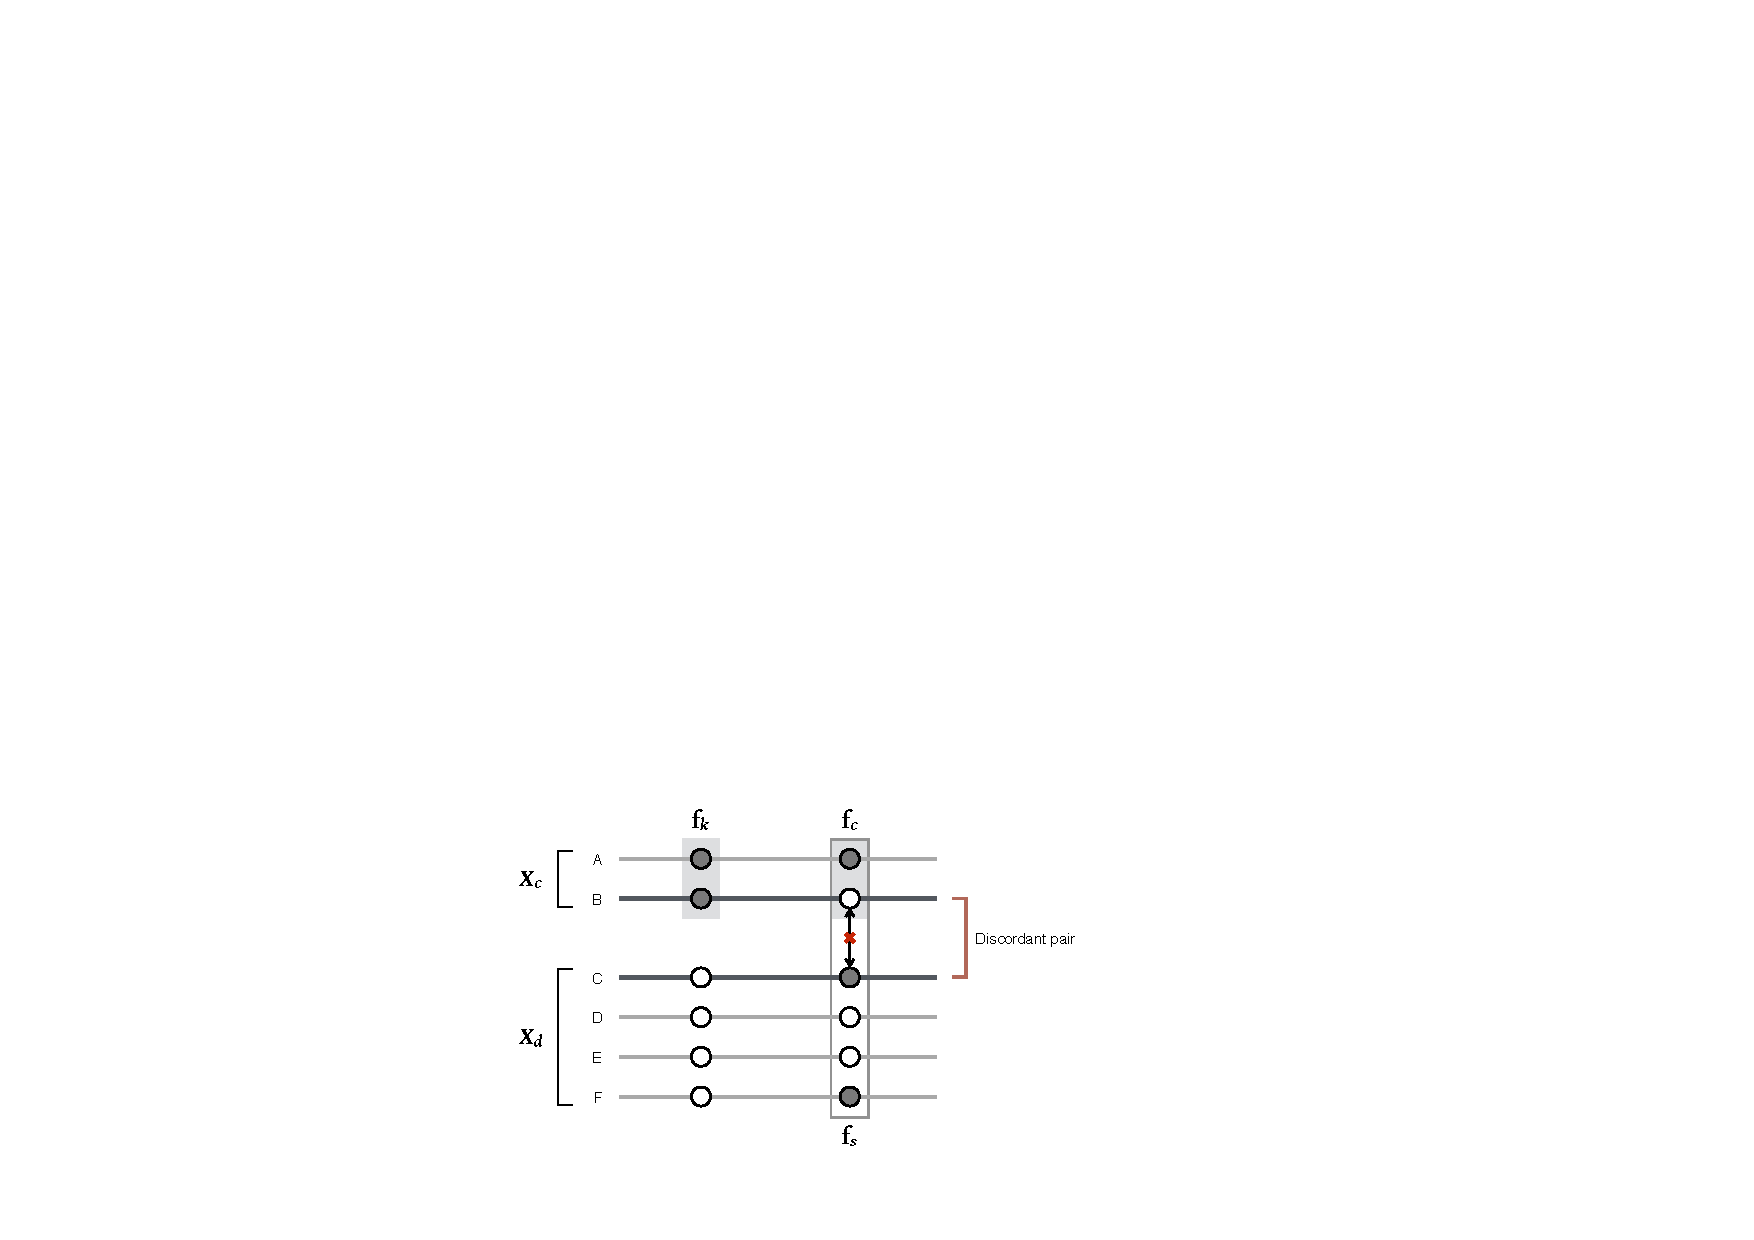
\includegraphics[width=0.7\textwidth]{./img/ch5/info_fgt_discord}
\Caption{Breakpoint detection in discordant pairs}%
{A discordant pair is formed by \n{1} haplotype from $X_c$ (which share the focal allele) and \n{1} haplotype from $X_d$ (which do not share the focal allele).
The lines indicate the chromosomal sequence where the alleles at \n{2} sites are indicated; allelic states are distinguished as the ancestral (\emph{hollow} circle) and derived state (\emph{solid}).
The conditions that lead to the detection of a recombination breakpoint is indicated between the focal site (\emph{left}) and another, distal site (\emph{right}), where \fk{} denotes the number of allele copies at the focal site within the subsample $X_c$, \fk{c} denotes the number of allele copies observed at the distal site within the subsample $X_c$, and \fk{s} denotes the number of allele copies at the distal site within the whole sample.
The \gls{fgt} is passed if all \n{4} allelic configurations are observed at \n{4} haplotypes in the sample.}%
{fig:info_fgt_discord}
\end{figure}
